\documentclass[Rapport/Playerside/RPI_IF/RPI_IF.tex]{subfiles}
\label{sec:playerside_RPI_IF_modultest}
\begin{document}
\subsubsection{Modultest}
Til modultest af RPI\_IF skulle I2c kommunikation til og fra PSoC'en testes. For at dette kunne lade sig gøre uden en funktionel RPI var, at bruge analog discovery, samt det tilhørende program waveforms, hvori der findes en protocol funktionalitet, hvor analog discovery kan bruges, som I2C master. I PSoC projektet bliver en UART tilføjet. Dette bliver gjort, da en masse stubs blev lavet for at teste med de funktioner, der bliver kaldt fra GameController klassen, men disse funktioner består kun af tekst udskrevet ved hjælp af UART komponenten. På denne måde kan vi i programmet tera term se de ting, der bliver udskrevet med UART. I figur \ref{fig:state_change} er alle states sendt til PSoC vist i terminalen, hvor vores stub for setState skriver den tilsvarende state ud til tera term via UART. Det samme er gjort i figur \ref{fig:color_change}, hvor det dog er farvekoden der sendes til PSoC'en. Her udskriver setMyColor og setOpponentColor stubs også de rigtige værdier for farvekoderne sendt, hvor farvekoden sendt for modstanderen er h01 h01 h01(tre hex værdier) og sin egen h02 h02 h02 i decimal er det henholdsvis 111 og 222.
\begin{figure}
    \centering 
    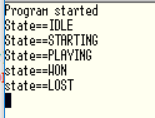
\includegraphics[width=0.5\linewidth]{Rapport/Playerside/graphics/RPI_IF/states.PNG}
    \caption{Alle states sendt til PSoC via I2C fra analog discovery.}
    \label{fig:state_change}
\end{figure}
\begin{figure}
    \centering 
    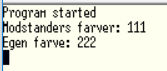
\includegraphics[width=0.5\linewidth]{Rapport/Playerside/graphics/RPI_IF/farvekode.PNG}
    \caption{Farvekode bliver sendt til PSoC via I2C fra analog discovery}
    \label{fig:color_change}
\end{figure}
Den sidste ting, der skulle testes, var om sendCupStatus fungerede ved at sende beskeder til analog discovery.  Hex værdien sendt er 3F hvilket også ses i figur \ref{fig:sendCupStatus}
\begin{figure}
    \centering 
    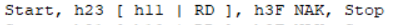
\includegraphics[width=0.5\linewidth]{Rapport/Playerside/graphics/RPI_IF/analog_read.PNG}
    \caption{Beskeden sendt fra PSoC modtages af analogdiscovery}
    \label{fig:sendCupStatus}
\end{figure}
For en mere uddybende beskrivelse af modultesten ses afsnit \fullref{sec:RPIIFmodultestbilag}
\end{document}
